\begin{rightcolumn}

\subsubsection*{Modalidad Greenfield} 

El valor del intangible es estimado usando las proyecciones de un flujo de efectivo que asume que el ÚNICO activo del negocio es el activo intangible bajo análisis. El resto de los activos necesarios deben ser comprados, construidos o rentados. Este método forma parte de los ``Differencial Value Methods'' (DVM) y son métodos de valuación del enfoque ingresos que estiman el valor de un activo mediante la comparación del negocio CON el activo y el negocio SIN el activo. (\ref{fig:greenfield})\\


En este caso el valuador llevó a cabo la aplicación del método de Flujo de Ahorro en Regalías en la modalidad Greenfield, al establecer que las regalías calculadas son el ÚNICO flujo de efectivo generado por la marca directamente al titular del activo intangible; en virtud de la(s) Licencia(s) de Marca(s) celebradas por el solicitante según quedó precisado en el \textcolor{principal}{APÉNDICE 2}.

\end{rightcolumn}

\begin{leftcolumn}

\begin{figure}[H]
\label{fig:rfr}\caption{Método Greenfield}
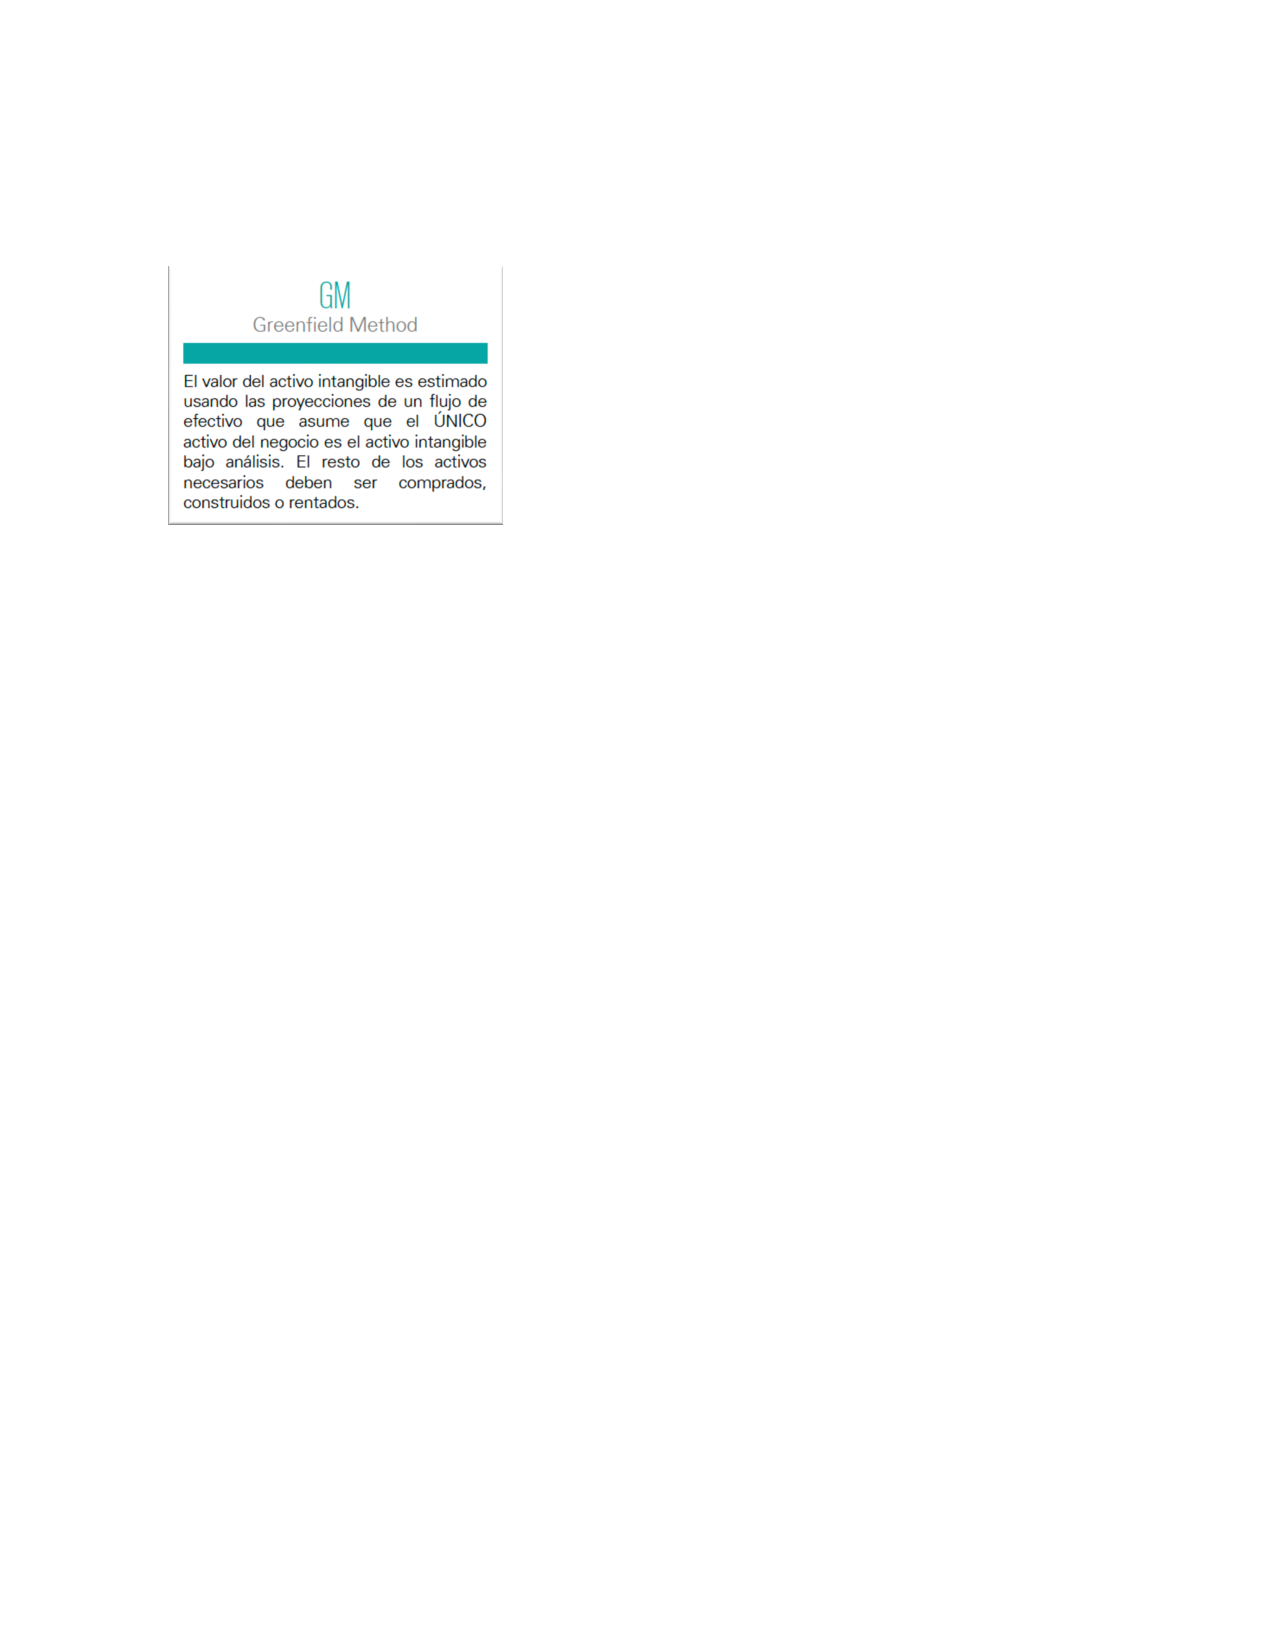
\includegraphics[width=\textwidth]{\rutaImagenes/greenfield_2}\\
\textit{Fuente: KPMG Cárdenas Dosal, S.C. Valuación de Activos Intangibles. Pag. 73. México, 2017.}
\end{figure}

\end{leftcolumn}